Um die Lichtverteilung in einer Szene vollständig zu beschreiben langt folgende Gleichung \ref{eq:Allgemeine Rendergleichung} \cite{kajiya1986rendering}

\begin{tcolorbox}[rightrule=3mm, rounded corners=east]
    \begin{equation}\label{eq:Allgemeine Rendergleichung}
        L(x,\omega) = L_{\epsilon}(x,\omega) + \int_{\Omega^{+}}f_{r}(\omega_{i},x,\omega)L_{i}(x,\omega_{i})*cos(\delta_{i})d\omega_{i}
    \end{equation}
\end{tcolorbox}

Die Strahldichte eines Punktes x in Richtung $\omega$ wird dabei maßgeblich von der grundsätzlich ausgesendeten Strahlung, dem Emissionsterm 
$L_{\epsilon}(x,\omega)$ sowie dem Integral über die positive Hemisphäre (für reine Reflexion; komplettes Sphärenintegral für zusätzliche 
Transmissionen) bestimmt. Dabei bestimmt das Integral jedwedes auf den Punkt x einfallendes Licht aus der Richtung $\omega_{i}$ und berechnet 
anhand der Reflektanzverteilungsfunktion $f_{r}$ seinen jeweiligen reflektierten Anteil in Richtung $\omega$. Da die Berechnung eines Integrals
über eine Hemisphäre unpraktikabel, wird zur photorealistischen Bildsynthese in aktuellen Anwendungen \cite{PathTracingInProduction} eine 
Monte-Carlo Integration gemacht.

\subsection{Monte-Carlo-Integration}
Mit der Monte Carlo Integration approximieren wir die Rendergleichung \ref{eq:Allgemeine Rendergleichung} bei gegebener Dimensionalität n des Renderintegrals 
(siehe auch \cite{KK02})

\begin{tcolorbox}[rightrule=3mm, rounded corners=east]
    \begin{equation}\label{eq:Monte-Carlo}
        \int_{a}^{b}f(x)dx \approx \frac{b-a}{N}\sum_{i=1}^{N}f(x_{i})
    \end{equation}
\end{tcolorbox}

Dabei wird das Integral \ref{eq:Allgemeine Rendergleichung} approximiert, indem wir die Funktion $f(x)$ an N zufälligen, uniform-verteilten
Stellen auswerten. 

\subsection{Funktionsweise}

Das Path Tracing ist eine Methode, die die Lichtverteilung durch Approximation des Hemisphären- mit Hilfe eines Monte-Carlo Integrals
\ref{eq:Monte-Carlo} löst. 

\begin{figure}[H]
    \begin{tcolorbox}
    \centering
    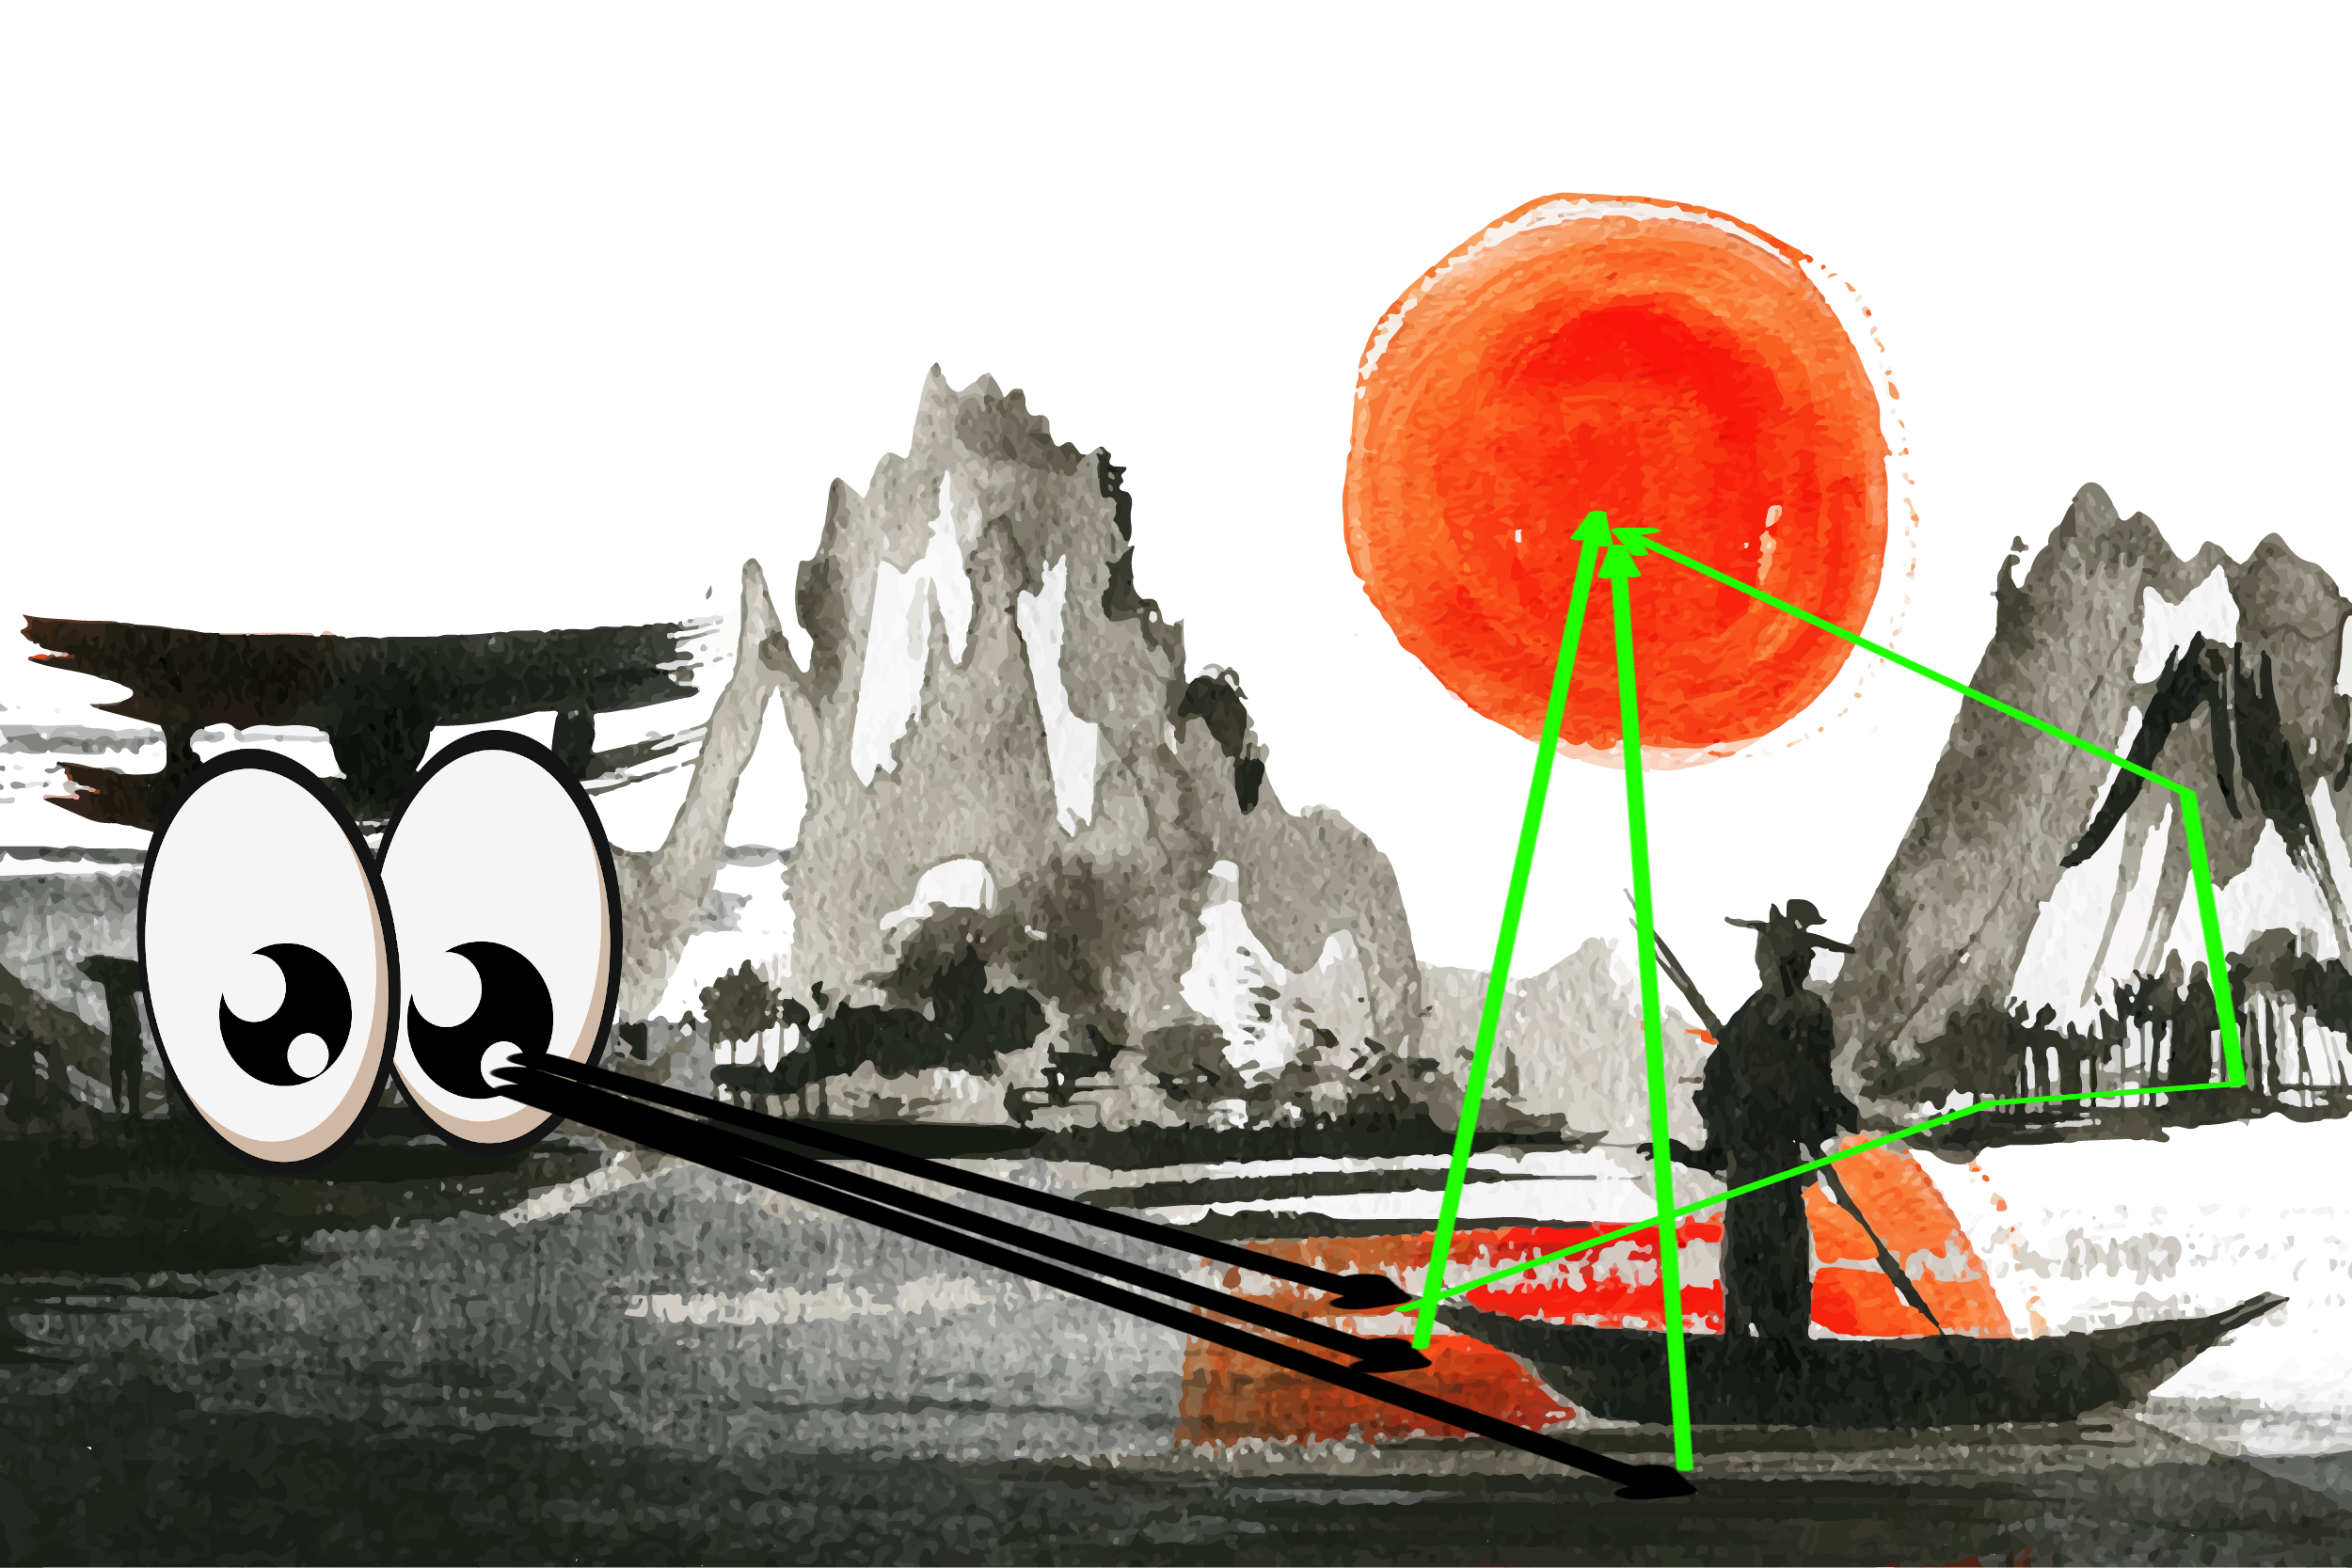
\includegraphics[width=\linewidth]{content/PathTracer/Bilder/PathTracerGuide.png}
    \end{tcolorbox}
    \caption{Sichtebene (blau), Sichtstrahlen(schwarz), Sekundärstrahlen(Schatten,Spiegelung,..) in grün}
    \label{pic::GrundkonzeptPathTracing}
\end{figure}

Zur Näherung werden hier nun für jeden Pixel mehrere Strahlen verschossen, welche jeweils nur einen Folgestrahl haben. Daher entstehen
mit dieser Methode pro Pixel mehrere einzelne Lichtpfade.
Der hier verwendete \nameref{ch:Content1:sec:Path Tracer} wurde mit dem Real-Time Rendering Framework Falcor \cite{Benty18} umgesetzt.

Klassischerweiße werden hierbei pro Pixel mehrere zufällige Strahlen verschossen, welche jeder 
für sich einen \textit{Samplewert} ergibt und zur Farbgebung des Pixels beiträgt. Mehrere
unkorrelierte zufällige Folgen ergeben somit die schlussendliche Pixelfarbe. Der Fehler, der 
bei der zugrundeliegenden Monte-Carlo Integration (siehe Gleichung \ref{eq:Monte-Carlo}) entsteht, 
wird klassischerweiße über Varianzreduktionsmethoden wie \textit{Importance Sampling}
angegangen.
Das Ziel hierbei ist es, die Fehlerverteilung im Bildraum zu beeinflussen, da diese für die wahrnehmbare 
visuelle Qualität des Bildes verantwortlich ist. Diese Arbeit wird vom diesen Vorgehen abweichen und direkt im 
Bildraum eine zeitlich stabile \nameref{ch:Content1:sec:blue noise}
Fehlerverteilung durch korrelierte Folgen erreichen. Die positive Auswirkung von \nameref{ch:Content1:sec:blue noise} 
Verteilungen auf die visuelle Qualität wurde bereits ausgiebig erforscht \cite{3288}.

\par 
\subsection{DirectX Raytracing}

\begin{figure}[H]
    \centering
    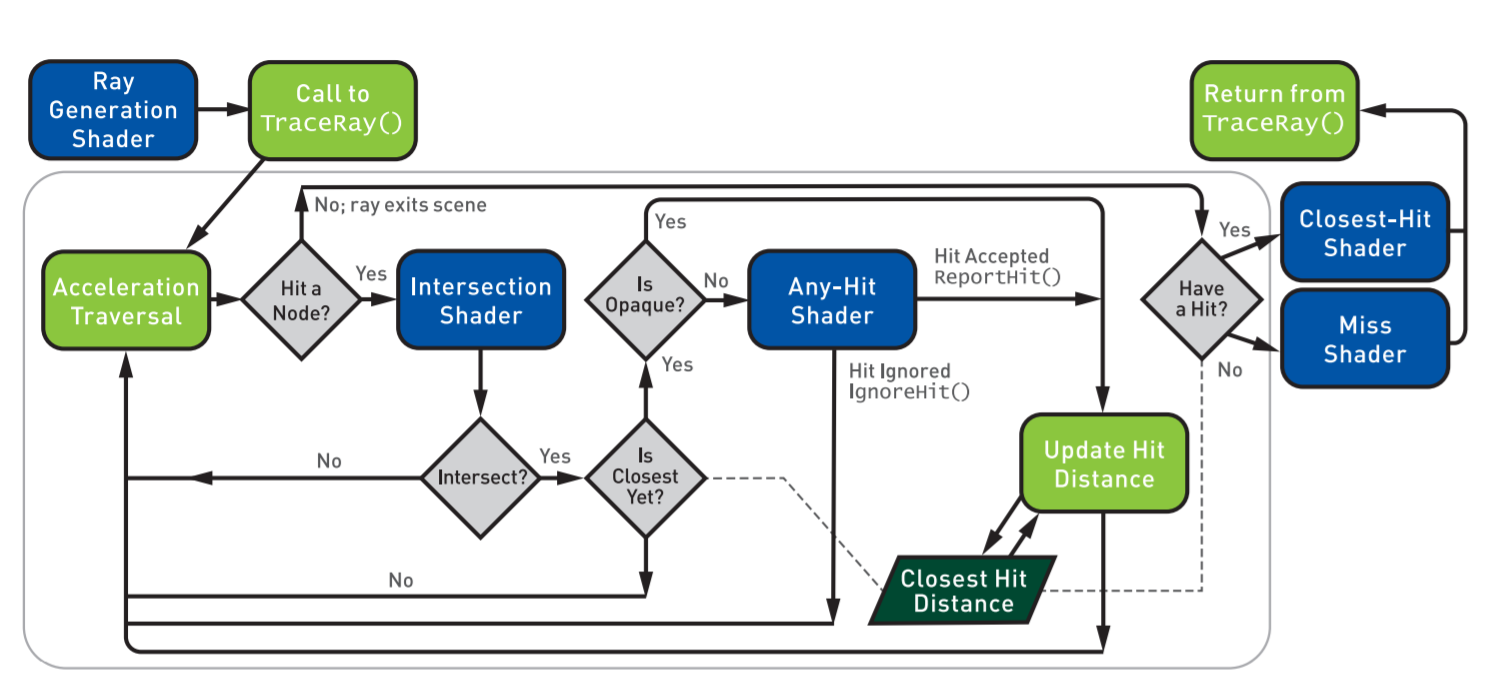
\includegraphics[width=\linewidth]{content/PathTracer/Bilder/DirectXRaytracingPipeline.png}
    \caption{DirectX Raytracing Pipeline aus \cite{Haines2019}}
    \label{pic:DirectXRaytracingPipeline}
\end{figure}

Das hardwareunterstützte Raytracing erhielt Einzug in moderne Programmierschnittstellen(DirectX, Vulkan) und wird 
hier anhand von DirectX erläutert, welche auch für die \textit{Global Illumination} innerhalb des 
Render Graphs \ref{pic:Render Graph} benutzt wurde. 

In Abbildung \ref{pic:DirectXRaytracingPipeline} und  Algorithmus \ref{alg:Path Tracer Konzept} lässt sich
der Beginn (Generierung eines Strahles) der neuen Pipeline durch den programmierbaren
\textbf{Ray Generation shader} erkennen.

\begin{tcolorbox}
\begin{algorithm}[H]
    \caption{Beispielhafter minimalistischer Ray Generation Shader}
    \begin{algorithmic}[1]
        \State [shader(\dq raygeneration \dq)]
        \State launchIndex = DispatchRaysIndex().xy;
        \For{(int i = 0; i < numberOfRays;i++)}
            \State float shadowRayMult = TraceRay(gRtScene,\par
            RAY\_FLAG\_ACCEPT\_FIRST\_HIT \_AND\_END\_SEARCH |\par
            RAY\_FLAG\_SKIP\_CLOSEST\_HIT\_SHADER,\par
            0xFF, 0, hitProgramCount, 0, ray, payload);
            \State float indirectRayColor = TraceRay(gRtScene, 0, 0xFF, 1, hitProgramCount,\par
            1, rayColor, payload);
            \State color = shadowRayMult * shadingColor \par
            + computeindirectLighting(indirectRayColor);
        \EndFor
        \State output[id] = color;
    \end{algorithmic}
    \label{alg:Ray Gen}
\end{algorithm}
\end{tcolorbox}

Mit Hilfe der Methode \textbf{TraceRay()} werden dann zur Beleuchtungsberechnung 
die Strahlen verschossen. Damit diese Methode richtig arbeiten kann übergeben wir neben unseren Strahl 
unter Anderem  unsere Szene inklusive Beschleunigungsstruktur, rayflags 
(beeinflussen Transparaenz, Culling, Abbruch)\cite{RayFlags} und einen payload.
Mit dem \textit{$payload_t$} können wir einen struct mit Informationen jedem einzelnen Strahl mitgeben.

\begin{tcolorbox}
\begin{algorithm}[H]
    \caption{beispielhafter payload}
    \begin{algorithmic}[1]
        \State struct RayPayload = {float4 color, uint32 seed, uint32 depth};        
        \end{algorithmic}
        \label{alg:payload}
\end{algorithm}
\end{tcolorbox}
    
Diese Methode \textbf{TraceRay()} kann auch innerhalb der anderen Shader zum weiteren verschießen
von Strahlen verwendet werden. So beispielweise beim Verschießen eines Schattenstrahls mit flags 
RAY\_FLAG\_ACCEPT\_FIRST\_HIT\_AND\_END\_SEARCH, \newline
RAY\_FLAG\_SKIP\_CLOSEST\_HIT\_SHADER setzen, um unnötige 
Beleuchtungsberechnungen und weitere Schnittpunktberechnungen zu umgehen und mit einem Bit als payload 
die Sichtbarkeit zur Lichtquelle mitzugeben.
Mit diesem beispielhaften payload können wir die Farbe akkumulieren, unsere  
seeds verwenden um z.B eine weiteren Strahlenschuss in einem Any-Hit Shader zu verwirklichen,  
solange die mit übergebene Rekursionstiefe in unserem payload eingehalten wird.  

\textbf{Intersection shader} führt die Schnittberechnungen durch.
Haben wir eine Szene, welche aus ausschließlich Dreiecken besteht, können wir
die auf Hardware standardmäßig gelieferte Implementierung übernehmen. 
Optionale Berechnungen für andere Geometrie können hier implementiert werden.
Bei einem gefundenen nähsten Schnittpunkt einer durchsichtigen Oberfläche wird der 
\textit{Any-hit shader} aufgerufen.
\textbf{Any-hit shaders} erlauben klassische \textit{Discards} oder informieren
über einen korrekten Schnitt. So können wir z.B. einen Alpha Test durchführen.

\begin{tcolorbox}
\begin{algorithm}[H]
    \caption{Any-Hit shader}
    \begin{algorithmic}[1]
        \State [shader(\dq anyhit \dq)]
        \If{(!alphaTest)} 
        \State IgnoreHit();
        \EndIf
    \end{algorithmic}
    \label{alg:any hit}
\end{algorithm}
\end{tcolorbox}

Der \textbf{Closest-hit shader} berechnet den Schnittpunkt des Strahls mit der Geometrie
der Szene, die dem Strahlursprung am nähesten ist.
Mit der Kennzeichnung [shader(\dq closesthit \dq)] wird die Hauptmethode zur 
dessen Ausführung markiert. An dieser Stelle bietet es sich an die Shading Farbe 
mit der Schnittpunktinformation zu aktualisieren und/oder um eine Rekursionstiefe weiter 
zu gehen einen weiteren Strahl zu verschießen. 
Der \textbf{miss shader} wird immer dann ausgeführt, wenn ein Strahl die
Szenengeometrie nicht schneidet. Kann also für das Nachschauen in einer 
Environment Map verwendet werden. 

Im Folgenden Algorithmus \ref{alg:Path Tracer Konzept} wird nochmal vereinfacht die Funktionsweise 
eines Path Tracers erläutert, wobei die entsprechenden programmierbaren Shader von DirectX 
im jeweiligen Codeabschnitt markiert sind.

\begin{tcolorbox}
\begin{algorithm}[H]
    \caption{Path Tracing Algorithmus}
    \begin{algorithmic}[1]
        \Procedure{Trace Path}{$BVH$}\Comment{verfolge Pfad durch Szene}
        \For{(x,y) $\in$ frame}
        \State strahl = verschiesseStrahlInPixel(x,y); // \textbf{ray generation shader}
        \For{blatt = bekommeBVHBlatt()}
        \State schnittpunkt = schneideGeometrie(strahl, blatt);\par
        //\textbf{Intersection shader}
        \If{schnittpunkt $\leq$ nähesterSchnittpunkt}
        \State aktualisiereNähestenSchnittpunkt();
        \EndIf
        \EndFor
        \If{Schnittpunkt gefunden}
        \State frame(x,y) = gebeFarbe(strahl,nähesterSchnittpunkt);\par
        //\textbf{closest-hit shader}
        \Else
        \State frame(x,y) = Umgebungskarte(x,y);//\textbf{miss shader}
        \EndIf
        \EndFor
        \EndProcedure
    \end{algorithmic}
    \label{alg:Path Tracer Konzept}
\end{algorithm}
\end{tcolorbox}

\subsection{Render Graph}

\begin{figure}[H]
    \begin{tcolorbox}
    \centering
    \def\svgwidth{\columnwidth}
    \import{content/PathTracer/Bilder/}{render_graph.pdf_tex}
    \end{tcolorbox}
    \caption{Render Graph}
    \label{pic:Render Graph}
\end{figure}

Für jeden Bilderzeugungsvorgang werden die in Abbildung \ref{pic:Render Graph} angegebenen Schritte von links nach rechts 
durchlaufen.








